\documentclass[journal,12pt,twocolumn]{IEEEtran}
\usepackage{tikz}
\usepackage{amsmath}
\usepackage{amssymb}
\pagestyle{empty}
\usepackage{setspace}
\usepackage{gensymb}
\singlespacing

\usepackage{amsmath}
\usepackage{amsthm}
\begin{document}
\newcommand{\myvec}[1]{\ensuremath{\begin{pmatrix}#1\end{pmatrix}}}
\newcommand{\cmyvec}[1]{\ensuremath{\begin{pmatrix*}[c]#1\end{pmatrix*}}}
\providecommand{\norm}[1]{\lVert#1\rVert}
\newcommand{\mydet}[1]{\ensuremath{\begin{vmatrix}#1\end{vmatrix}}}
\newcommand{\proj}[2]{\textbf{proj}_{\vec{#1}}\vec{#2}}
\let\StandardTheFigure\thefigure
\let\vec\mathbf

\title{
Assignment - 1
}
\author{ LAKSHMI GAYATHRI GUDIPUDI - SM21MTECH11001}
\maketitle
\newpage
\bigskip
\bibliographystyle{IEEEtran}
\section*{\textbf{Problem}}
\noindent


Find the Area of Quadrilateral when four points are given
\begin{align}
\vec{P} = \myvec{2\\1}, \vec{Q} =\myvec{3\\5},
\vec{R} =\myvec{-3\\4}, \vec{S} =\myvec{-2\\-2}
\end{align}

\noindent
\section*{\textbf{Solution}}
\noindent

Area of a Quadrilateral PQRS is 
\begin{align}
Area (\Delta PQR)+ Area (\Delta PRS)
\end{align}
\begin{align}
Area (\Delta PQR)=
$$\frac{1}{2}\norm{(\vec{Q}-\vec{P})\times(\vec{Q}-\vec{R})}
\end{align}
For two vectors \vec{a}=\myvec{a1\\a2} and \vec{b}=\myvec{b1\\b2}
\begin{align}
\norm{\mathbf{\vec{a}\times\vec{b}}}=|a1b2-a2b1|
\end{align}
$$\vec{Q-P}=\myvec{1\\4}

$$\vec{Q-R}=\myvec{6\\1}

\begin{align}
Using Area (\Delta PQR)=
$$\frac{1}{2}\norm{\mathbf{(\vec{Q}-\vec{P})\times(\vec{Q}-\vec{R})}}
\end{align}

\begin{align}
$$=\frac{1}{2}\left|(-23)\right|
\end{align}

Similarly 
\begin{align}
Area of (\Delta PRS)=
$$\frac{1}{2}\norm{\mathbf{(\vec{S}-\vec{P})\times(\vec{S}-\vec{R})}}
\end{align}

$$\vec{S-P}=\myvec{-4\\-3}

$$\vec{S-R}=\myvec{1\\-6}

\begin{align}
Using Area of (\Delta PRS)
$$=\frac{1}{2}\norm{\mathbf{(\vec{S}-\vec{P})\times(\vec{S}-\vec{R})}}
$$=\frac{1}{2}|(27)|
\end{align}

So total area of Quadrilateral PQRS is 
\begin{align}
Area (\Delta PQR)+Area (\Delta PRS)
\end{align}

\begin{align}
$$=\frac{1}{2}|(-23)|+\frac{1}{2}|(27)|
\end{align}

\begin{align}
$$=(23+27)/2
\end{align}

\begin{align}
$$=25 sq.units
\end{align}

\begin{figure}[!ht]
    \centering
    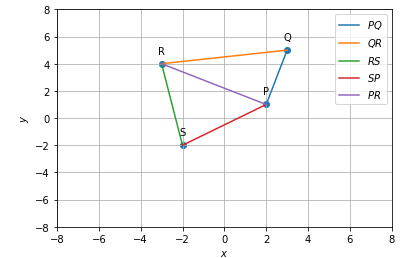
\includegraphics{QUAD.PNG}
    \caption{Quadrilateral PQRS}
    \label{fig:Quad Figure}
\end{figure}


\end{document}

